\documentclass{article}
\usepackage[utf8]{inputenc}
\usepackage[document]{ragged2e}
\usepackage{algpseudocode}
\usepackage[]{algorithmicx}
\usepackage{amsmath}
\usepackage{amsthm}
\usepackage{amssymb}
\usepackage[]{listings}
\usepackage{graphicx}
\usepackage{hyperref}
\usepackage{flafter}
\usepackage{subfig}
\usepackage{dsfont}
\graphicspath{ {images/} }

\begin{document}

\begin{titlepage}
	\centering
	
\includegraphics[width=0.15\textwidth]{IIIT-B_logo.jpg}\par\vspace{1cm}
	{\scshape\LARGE International Institute of Information Technology, Bangalore \par}
	\vspace{1cm}
	{\scshape\Large Project Strategy Document\par}
	{\Large  DS 707 Data Analytics\par}
	\vspace{1.5cm}
	{\huge\bfseries Exploratory Analytics and Classification \par}
	\vspace{2cm}
	{\Large\itshape Akanksha Dwivedi - MT2016006\par}
	{\Large\itshape Hitesha Mukherjee - MS2016007\par}
	{\Large\itshape Nayna Jain - MS2017003\par}
	{\Large\itshape Tarini Chandrashekhar - MT2016144\par}
	\vfill
	Instructors : \par
	Prof. Ramanathan Chandrashekhar
	\par
	Prof. Uttam Kumar

	\vfill
% Bottom of the page
	{\large \today\par}
\end{titlepage}

\newpage

\tableofcontents

\newpage
\justify


\section{Data Exploration}

\subsection{Select Classification
Technique }
Following the paper "Automatic Bitcoin Trading via Machine Learning Algorithms"" by Isaac Madan, Shaurya Saluja and Aojia Zhao, we manually select 16 features, namely:
\begin{itemize}
\item Average Confirmation Time Block Size
\item Cost per transaction percent Difficulty
\item Estimated Transaction Volume Hash Rate
\item Market Capitalization
\item Miners Revenue
\item Number of Orphaned Blocks Number of TXN per block Number of TXN
\item Number of unique addresses Total Bitcoins
\item TXN Fees Total
\item Trade Volume Transaction to trade ratio
\end{itemize}

Names and descriptions of the 16 features we chose that relate to the Bitcoin network. We leveraged these features in developing a binary and a ternary classification algorithm to predict the sign change in Bitcoin price based on daily data points. The binary classification algorithm predicts positive and no change as 1 and negative price change as -1. The ternary classification algorithm predicts positive price change as 0, negative price change as -1, and no change as 0. We used the results of the following classification algorithms, and compared their results. We got less accuracy as compared to the paper. Our data is a date wise data, while they used a 24-hour data, taken from coinexchange:

Another technique that is applied is simple linear regression on bitcoin price data was to predict Open Price based on Market Capitalization. Linear Regression is used for predictive analysis. In this case, there is a response variable whose outcome has to be predicted based on the input variables which are also called as dependent variables. Linear Regression is used with continuous type of data. 

Further, Cryptocurrency data is similar to stock analysis data. As discussed in paper by Luckyson, Snehasu, Sudeepa, Random Forest has been used to predict the stock prices.
Random Forest is an ensemble learning method for classification and regression by considering lot of decision trees at training time and specifying the class based on the mode of the classes as identified by different trees.
Here the Random Forest is applied on bitcoin\_dataset to predict the bitcoin market price.

\begin{itemize}
\item Multinomial Regression  -
\item Naives Bayes		      -
\item Random Forest.             -
\item SVM 		
\item Linear Regression              -
 \end{itemize}

\subsection {Build Classification Model Parameter Setting}

\subsubsection{Linear Regression}
We have prepared a simple model of estimating Open Prices based on Market Capitalization. The independent variable is Market Capitalization and estimation is done for Open Price.

\subsection {Visualizing Using Tableau}
We explored the variation of various attributes of cryptocurrencies and their impact on their use worldwide. 
\begin{itemize}

\item The hash rate of a cryptocurrency is a measure of how many proof of work calculations are being performed by all the miners participating in the network. It is measured in terms of hashes per second, but because such as large number of these calculations are performed it is more usual to see values in larger units such as Gigahashes per second (GHS) or Terrahashes per second (THS).

That means, if a cryptocurrency network has a low hash rate then the cost for an attacker wanting to purchase enough hashing power to attack the network would be relatively low. As the hash rate goes up, so does the cost of attacking the network.

\item There is a long-run feedback cycle between difficulty and price. If price goes up, that makes mining more lucrative, and people buy new hardware to capitalize on that. As hashing power increases as a result, however, there’s actually a temporary increase in the daily bitcoin production, thereby causing an increase in the supply. This occurs because difficulty only adjusts every 2016 blocks, so as mining power increases it takes difficulty some time to catch up – and in the meantime, blocks are produced more frequently than once per 10 minutes target rate.

\item When the number of transaction increases, When number of transactions increase more blocks are produced. Since there is a cap of average 1 block per 10 minutes the difficulty of the network increases. With the difficulty increase hashrate has to increase to keep generating blocks on time.

\item When hashrate increases, the difficulty increases as well because with number of transactions increasing hashrate has to increase to keep processing them. With the hashrate increased blocks are generate faster and thus difficulty is increased.

\end{itemize}

\subsection {Assessing the  Classification Model Built}

\subsubsection{Linear Regression Model}

The mean square error which we got was  0.2127196982. It seems to be doing average estimation

Chart below shows the predicted vs actual value.

\begin{figure}
	\centering
	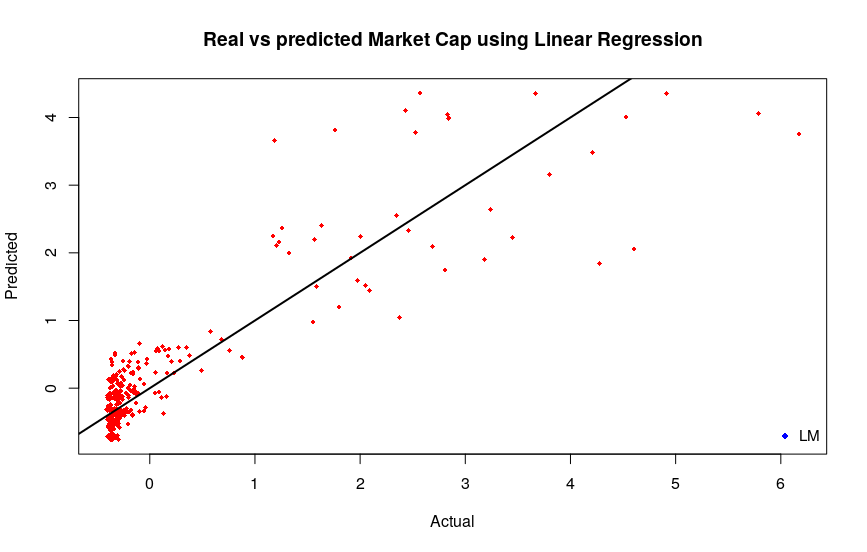
\includegraphics[width=\linewidth]{charts/bitcoin_market_cap_using_LR}
	\caption{Bitcoin Market Cap Prediction based on Open Price}
	\label{fig:Bitcoin Market Cap Prediction}
\end{figure}

\begin{thebibliography}{References}
	\bibitem{1}
	Predicting the direction of stock market prices
	using random forest. Luckyson Khaidem Snehanshu Saha Sudeepa Roy Dey. khaidem90@gmail.com snehanshusaha@pes.edu sudeepar@pes.edu
	
\end{thebibliography}


\end{document}
